\documentclass{article}
\usepackage{fullpage}
\usepackage{graphicx}
\usepackage{url}
\begin{document}

\title{XXBX Power Shim-XBP User Guide}

\maketitle

\section{XBP Configuration}
The XBP uses three voltage supplies. The first supply, called $\mathrm{V_{CC}H}$
uses 3.3\,V from the XBH and powers the I$^2$C pull-up resistors, the activity LED, 
and the level shifters.
The second supply, called $\mathrm{V_{CC}P}$ uses 5\,V and powers the current
sense amplifier of the XBP and the power LED. 
The third supply is $\mathrm{V_{CC}D}$ which powers the XBD.

\subsection{Powering the XBP}
In this section we only discuss how to supply $\mathrm{V_{CC}H}$ and $\mathrm{V_{CC}P}$.
There are two options to power the XBP. Option one is to power the XBP from the
XBH using the LaunchPad connector. This only works if the XBP is directly plugged into the 
LaunchPad connector on the XBH, 
we call this an XBP0. Then the XBH can supply $\mathrm{V_{CC}H}$ and $\mathrm{V_{CC}P}$.
Please close solder jumper \textbf{SJ4} and solder jumper \textbf{SJ5} and do not connect
the power connector's $\mathrm{V_{CC}H}$ and $\mathrm{V_{CC}P}$ pins to the XBH. 
They can be used to power another XBP though.

The other option is to power the XBP through the power connector on the front 
(see Fig.~\ref{fig:power}). This works for XBP0 through XBP3. Please make sure that the
solder jumper \textbf{SJ4} and solder jumper \textbf{SJ5} are \textbf{open}. 
$\mathrm{V_{CC}H}$ of 5\,V and $\mathrm{V_{CC}P}$ of 3.3\,V can be wired to the 
corresponding pins on the XBH or the power connector of the XBP0 if the XBP0 is supplied directly from the
XBH through the LaunchPad connectors.


\begin{figure}[ht]
  \begin{center}
    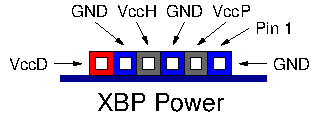
\includegraphics[scale=1]{figures/xbp_power}
    \caption{XBP Power Connector as Viewed from Front of PCB}\label{fig:power}
  \end{center}
\end{figure}

\subsection{Powering the XBD}\label{sec:vccd}
Power for the XBD can be provided through the power connector's $\mathrm{V_{CC}D}$ pin.
Optionally $\mathrm{V_{CC}D}$ can be generated on the XBP from the 5\,V $\mathrm{V_{CC}P}$.
If this is desired, please populate \textbf{IC1} with an LDO voltage regulator in a 
SOT-89-3 package. An example is the Microchip MCP1702T-3302E/MB 3.3\,V regulator.


\subsection{I$^2$C Pull-Up Resistors}
The XBP can provide the pull-up resistors for I$^2$C. These are needed only once on an 
I$^2$C bus. We suggest that you populate \textbf{R3} and \textbf{R4} using 
10\,kOhm resistors (size: 0604) on the first XBP (XBP0).

\subsection{Using XBDs with V$_{CC} = 3.3$\,V}
If your XBD uses a V$_{CC} = 3.3$\,V and has a LaunchPad connector, you can plug it 
directly on top of the XBP. 
Otherwise you can use the XBD connector on the back of the XBP (see Fig.~\ref{fig:xbd})
and close solder jumpers \textbf{SJ1}, \textbf{SJ2}, and \textbf{SJ3} as you
don't need voltage level shifting.
In either case, please check Section~\ref{sec:xbd} in this guide for details
on particular XBDs. 

\begin{figure}[ht]
  \begin{center}
    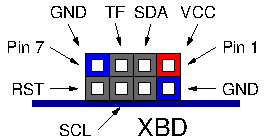
\includegraphics[scale=1]{figures/xbd_connector}
    \caption{XBD Connector as Viewed from Back of PCB}\label{fig:xbd}
  \end{center}
\end{figure}

\subsection{Using XBDs with V$_{CC} \not= 3.3$\,V}
Such XBDs can only be connected through the XBD connector on the back (Fig~\ref{fig:xbd}).
The FETs Q3 through Q8 and the resistors R9  through R11 have to be populated.
Please make sure that solder jumpers \textbf{SJ1}, \textbf{SJ2}, and \textbf{SJ3} 
are open. $\mathrm{V_{CC}D}$ can be higher or lower than 3.3\,V.

\subsection{Usage without XBH}
The XBP can be used also without an XBH as an experimenter's board for the INA225 
current sense amplifier. The XBH requires $\mathrm{V_{CC}P}$ of 5\,V to be supplied
through its power connector (see Fig.~\ref{fig:power}. The power for the device 
under test can be supplied as described in section~\ref{sec:vccd}. The amplified
voltage drop over the shunt can be measured by through the SMA connector \textbf{X1}.
The gain of the amplifier can be set through jumper JP5. The jumper settings required
for the different gains are printed on the circuit board. The device under test will
get its power from the XBD connector (see Fig.~\ref{fig:xbd}). Only pins 1 and 2,
V$_{CC}$ and GND respectively, have to be used.

\section{XBX Devices under Test (XBD)}\label{sec:xbd}
\subsection{TI Stellaris\textregistered~LM4F120 LaunchPad}

Neither the Debug, nor the Device USB should be connected for power measurements.
The \emph{+3.3V} line on pin J1.1 of the boosterpack connector is connected 
directly to the In-Circuit Debugger. Therefore, it is recommended to select on the
XBP to power the XBD via the external XBD connector and not via the boosterpack
connector. On the TI Stellaris Launchpad, the VDD jumper has to be pulled and the
external 3.3V has to be supplied to the right pin. The green power LED on the
Launchpad lights up when the 3.3V are supplied to the left (wrong) pin. 
The \emph{PWR Select} switch can be in any position and won't affect the 
measurements.

\subsection{TI Tiva\texttrademark~C Series TM4C123G LaunchPad}

The circuit connections are the same as on the TI Stellaris LaunchPad. Please follow
those instructions. Supply voltage is 3.3V with a maximum current of 300\,mA.

\subsection{TI MSP430F5529 LaunchPad\texttrademark}

For precise current measurements remove all jumpers from the isolation jumper block 
with the exception of the ground (GND) jumper. 

\subsection{TI MSP430FR6989 LaunchPad\texttrademark}

For precise current measurements remove all jumpers from the isolation jumper block 
with the exception of the ground (GND) jumper. Supply voltage is 3.3V with a maximum 
current of 2.7\,mA not including LEDs or external circuitry.

\section{XBP Assembly}

\section{XBP Connections}

\begin{figure}[ht]
  \begin{center}
    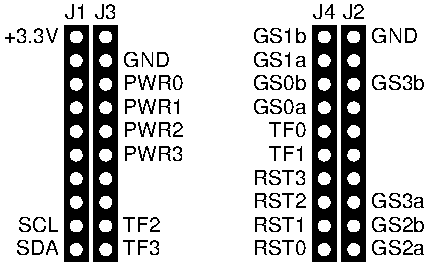
\includegraphics[scale=1]{figures/xbp-xbh}
    \caption{Boosterpack Connector XBH as Viewed from Top of PCB}
  \end{center}
\end{figure}

\begin{figure}[ht]
  \begin{center}
    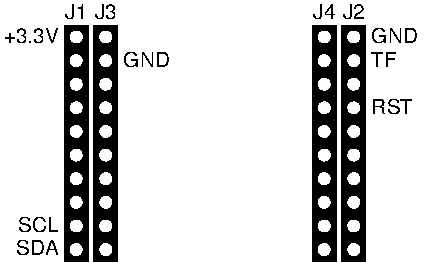
\includegraphics[scale=1]{figures/xbp-xbd}
    \caption{Boosterpack Connector XBD as Viewed from Top of PCB}
  \end{center}
\end{figure}
\begin{table}[ht]
  \begin{center}
    \caption{Pin Configuration of Boosterpack Connector for XBH}
    \begin{tabular}{rlll}
      Connector & Pin  & Net         & Comment  \\ \hline
       J1 & 1  & +3V3      & Supply Voltage $\mathrm{V_{CC}H}$ from XBH for I$^2$C pull-up resistors on XBP0 \\
       J1 & 9  & SCL       & I$^2$C Serial Clock  \\
       J1 & 10 & SDA       & I$^2$C Serial Data \\ 
       J3 & 21 & +5V       & Supply Voltage $\mathrm{V_{CC}P}$ from XBH for the XBP0 \\ \hline

       J3 & 23 & PWR0      & Analog signal of current consumption of XBD0 from XBP0\\
       J4 & 37/38 & GS0a/GS0b & Gain select for current monitor of XBD0 on XBP0\\
       J4 & 36 & TF0       & Timer Flag from XBD0 \\
       J4 & 31 & RST0      & Reset of XBD0 \\ \hline

       J3 & 24 & PWR1      & Analog signal of current consumption of XBD1 from XBP1 \\
       J4 & 39/40 & GS1a/GS1b & Gain select for current monitor of XBD1 on XBP1\\
       J4 & 35 & TF1       & Timer Flag from XBD1 \\
       J4 & 32 & RST1      & Reset of XBD1 \\ \hline

       J3 & 25 & PWR2      & Analog signal of current consumption of XBD2 from XBP2 \\
       J2 & 11/12 & GS2a/GS2b & Gain select for current monitor of XBD2 on XBP2\\
       J3 & 29 & TF2       & Timer Flag from XBD2 \\
       J4 & 33 & RST2      & Reset of XBD2 \\ \hline

       J3 & 26 & PWR3      & Analog signal of current consumption of XBD3 from XBP3 \\
       J2 & 13/18 & GS3a/GS3b & Gain select for current monitor of XBD3 on XBP3\\
       J3 & 30 & TF3       & Timer Flag from XBD3 \\
       J4 & 34 & RST3      & Reset of XBD3 \\ \hline

       J2 & 20 & GND       & \\
       J3 & 22 & GND       & \\ \hline
    \end{tabular}
  \end{center}
\end{table}
\begin{table}[ht]
  \begin{center}
    \caption{Pin Configuration of Boosterpack Connector for XBD}
    \begin{tabular}{rlll}
      Connector & Pin  & Net         & Comment  \\ \hline
       J1 & 1  & +3V3      & Supply Voltage, current is measured by XBP \\
       J1 & 9  & SCL       & I$^2$C Serial Clock  \\
       J1 & 10 & SDA       & I$^2$C Serial Data \\
       J2 & 16 & RST       & Reset of XBD \\ 
       J2 & 19 & TF        & Timer Flag to start/stop execution timer on XBH \\
       J2 & 20 & GND       & \\
       J3 & 22 & GND       & \\ \hline
    \end{tabular}
  \end{center}
\end{table}



\end{document}
